\documentclass[10pt,titlepage,a5paper]{ltjsbook}
\usepackage{amsmath}
\usepackage{amssymb}
\usepackage{amsfonts}
\usepackage{graphicx}
\usepackage{float}
\usepackage{xcolor}
\usepackage{enumitem}
\usepackage{etoolbox}
\usepackage{subfiles}
\usepackage{cleveref}
\usepackage{tcolorbox}
\usepackage{quotchap}
\usepackage{fancyhdr}
\usepackage{wrapfig}
\usepackage{geometry} % geometry パッケージを読み込む
\geometry{
    a5paper,      % 用紙サイズを再度指定(冗長でも安全のため)
    left=12mm,    % 左の余白を12mmに
    right=12mm,   % 右の余白を12mmに
    top=12mm,     % 上の余白を12mmに
    bottom=12mm,  % 下の余白を12mmに
    %showframe % 余白の境界線を可視化したい場合(最終出力時には削除)
}
\usepackage{titlesec}
\titleformat{\section}[block]{}{}{0pt}
{
  \definecolor{teal}{gray}{0.30}
  \begin{picture}(0,0)
    \put(-10,-5){
      \begin{tikzpicture}
        \fill[teal] (0pt,0pt) rectangle (5pt,19pt);
      \end{tikzpicture}
    }
    \put(-10,-5){
      \color{teal}
      \line(1,0){\hsize}
    }
  \end{picture}
  \hspace{0pt}
  \sffamily \Large \thesection
  \hspace{0pt}
}
\pagestyle{fancy} % fancy スタイルを使用することを宣言

% ヘッダーとフッターのすべてのフィールドをクリア
\fancyhf{}

% 奇数ページ (odd page) のフッター設定
\fancyfoot[LO]{\thepage} % Left Odd: 左下 (ページ番号)
\fancyfoot[RO]{}         % Right Odd: 右下 (空にする)

% 偶数ページ (even page) のフッター設定
\fancyfoot[LE]{}         % Left Even: 左下 (空にする)
\fancyfoot[RE]{\thepage} % Right Even: 右下 (ページ番号)

% ヘッダーとフッターの下線を消す
\renewcommand{\headrulewidth}{0pt} % ヘッダーの下線を0pt (消去)
\renewcommand{\footrulewidth}{0pt} % フッターの上線を0pt (消去)

% chapter の開始ページ(plain スタイル)もフッターにページ番号を表示させる
\fancypagestyle{plain}{
  \fancyhf{} % ヘッダーとフッターをクリア
  \fancyfoot[LO]{\thepage} % 左下 (奇数ページ)
  \fancyfoot[RE]{\thepage} % 右下 (偶数ページ)
  \renewcommand{\headrulewidth}{0pt} % ここにも下線消去を設定
  \renewcommand{\footrulewidth}{0pt} % ここにも下線消去を設定
}
\begin{document}
%\chapter{屋久島の地理}
  \section{位置と大きさ}
    屋久島は九州本土最南端の佐多岬から南南西約60kmの海上に位置する離島である. 船で向かう途中, 屋久島の姿が見えてくると, その見た目はまるで巨大な山である. 屋久島は洋上アルプスの異名を持ち,
    1700m級の山が7座, 1000mを超える山が45座連なっている. \\
    その大きさは約504$\mathrm{km^2}$, 周囲約132 kmであり, ほぼ円形の島である.
  \section{地質と形成}
    \begin{minipage}{0.38\columnwidth}
      \begin{figure}[H]
        \centering
        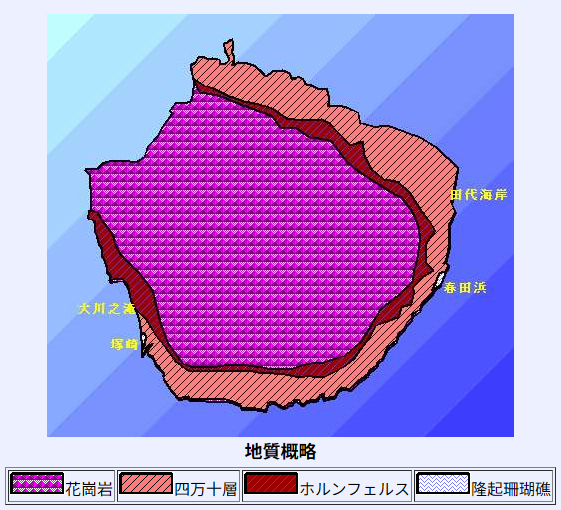
\includegraphics[width=\columnwidth]{yakushima_geology.png}
        \caption{屋久島の地質図}
        \label{fig:yakushima_geology}
      \end{figure}
    \end{minipage}
    \hfill
    \begin{minipage}{0.58\columnwidth}
      屋久島の地質は外周部が日向群層の堆積岩からなり, 中央部に直径約25kmの花崗岩が貫入している. この花崗岩は約1550万年前に地下のマグマだまりから形成され, その後花崗岩が隆起したことによって屋久島の高い山々ができたとされている.
      実はこの花崗岩との違いが隣の平坦な種子島との違いを生んでいる.堆積岩と花崗岩の接点部分は熱変性によりホルンフェルスになっている. ホルンフェルスは非常に硬く, 屋久島の滝を形成する一因となっている.
      このホルンフェルスの沿ってタングステンの鉱脈が存在し, 鉱山跡が点在している.
      一方, 春田浜や栗生の塚崎には隆起サンゴ礁の海岸が広がっている.
    \end{minipage}
    \vspace{2em}
    \begin{tcolorbox}[title=コラム:屋久島の花崗岩,width=\textwidth]
      \begin{minipage}{0.34\columnwidth}
        \begin{figure}[H]
          \centering
          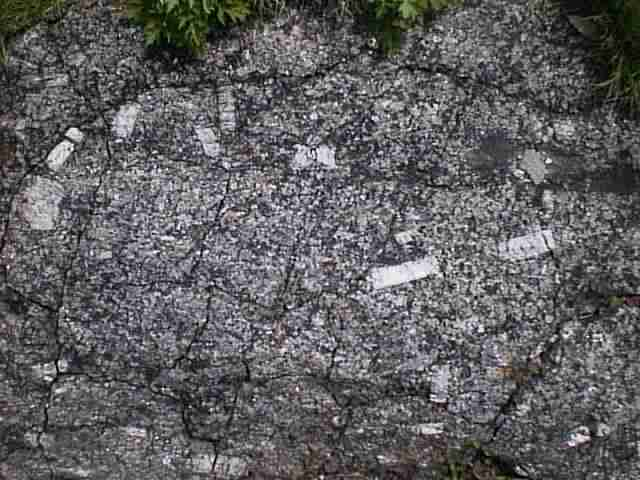
\includegraphics[width=\columnwidth]{kakougan.jpg}
          \caption{屋久島の花崗岩}
          \label{fig:yakushima_granite}
        \end{figure}
      \end{minipage}
      \hfill
      \begin{minipage}{0.64\columnwidth}
      屋久島の花崗岩は, 大きな正長石の結晶を含むので, 白っぽく見える. これはマグマがゆっくり固まったためだといわれている. 花崗岩は浸食されやすく, 屋久島の高山では風化した特徴的な形の花崗岩\footnotemark を見ることができる. 
      \end{minipage}
    \end{tcolorbox}
    \footnotetext[1]{屋久島の名所にて後述}
    \subsection*{幸谷火砕流}
      \begin{minipage}{0.33\columnwidth}
        \begin{figure}[H]
          \centering
          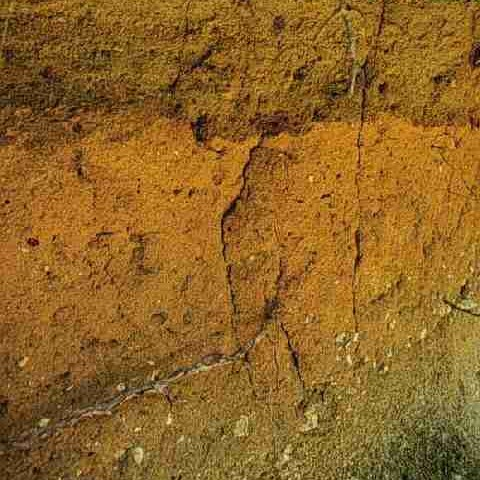
\includegraphics[width=\columnwidth]{kasairyu.jpg}
          \caption{幸谷火砕流}
          \label{fig:yakushima_kouya}
        \end{figure}
      \end{minipage}
      \hfill
      \begin{minipage}{0.6\columnwidth}
        屋久島の地層を見てみると, 幸谷火砕流と呼ばれる火山灰の層がある. これは屋久島の北約40kmにある鬼界カルデラが7300年前に噴火した際に飛散した火砕流であり, 幸谷火砕流と呼ばれている.
        この火山灰は東北地方まで飛散している. 屋久島全域でこの層は見られ\footnotemark, 厚さは数十cmから2m以上あり, 島中が火砕流に覆われたことがわかる. \\
        屋久島という花崗岩からできた貧栄養の島が幸谷火砕流によって栄養を得たことは, 屋久島の豊かな森の形成に影響を与えたであろうことは間違いない.
      \end{minipage}
      \footnotetext[2]{泊まるところの近くにみられる場所があるので, 授業と称して車を停めることになろう.}
  \section{荘厳な山々と水の恵み}
    \subsection*{屋久島の山々}
      \begin{minipage}{0.38\columnwidth}
      \begin{figure}[H]
        \centering
        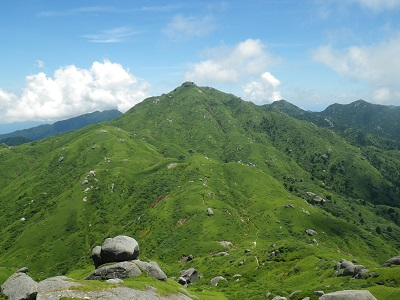
\includegraphics[width=\columnwidth]{mt_miyanoura1.jpg}
        \caption{宮之浦岳}
        \label{fig:yakushima_mountains}
      \end{figure}
      \end{minipage}
      \hfill
      \begin{minipage}{0.58\columnwidth}
        屋久島には数多くの山があり, その中でもとくに有名なものを挙げると,
        \begin{itemize}
          \item 九州最高峰の宮之浦岳(1936m)\footnotemark[3]
          \item 九州 第二峰の永田岳(1886m)\footnotemark[3]
          \item 黒味岳(1831m)\footnotemark[3]
          \item 山頂に巨大な岩(天柱石)がある太忠岳(1497m)
          \item 巨大な一枚岩からなるモッチョム岳(944m)
        \end{itemize}
      \end{minipage}
      \footnotetext[3]{この三座(黒味岳が栗生岳の場合もある)は屋久島の三岳と呼ばれている.}
    \subsection*{河川と滝}
      屋久島には多くの河川と滝が存在し, その中でも特に有名なものを挙げると,
      \begin{minipage}{0.38\columnwidth}
        \begin{figure}[H]
          \centering
          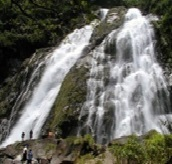
\includegraphics[width=\columnwidth]{okotaki.jpg}
          \caption{大川の滝}
          \label{fig:yakushima_river}
        \end{figure}
      \end{minipage}
      \begin{minipage}{0.58\columnwidth}
        \begin{itemize}
          \item 宮之浦川:屋久島最大級の河川で, 今回何度も入ることになるだろう.
          \item 安房川: 安房集落にある川で, 汽水域\footnotemark[4] が長く, カヌーSUPができる.
          \item 栗生川: 栗生集落にある川で, 河口にメヒルギのマングローブ林がある. 
          \item 大川の滝: 屋久島最大の滝で, 高さ88mの大迫力の滝.
          \item 千尋の滝: 大きな一枚岩の間を流れる滝. 
        \end{itemize}
      \end{minipage}
      \footnotetext[4]{淡水と海水が混ざり合う場所}
\end{document}